\documentclass[conference]{IEEEtran}
\usepackage{amsmath,amssymb,amsfonts}
\usepackage{algorithmic}
\usepackage{graphicx}
\usepackage{textcomp}
\usepackage{xcolour}
\usepackage[backend=biber, sorting=none]{biblatex}
\usepackage{url}
\usepackage{subcaption}
\usepackage[colorlinks=true, urlcolor=blue, pdfborder={0 0 0}]{hyperref}
\addbibresource{bibliography.bib}
\def\BibTeX{{\rm B\kern-.05em{\sc i\kern-.025em b}\kern-.08em
    T\kern-.1667em\lower.7ex\hbox{E}\kern-.125emX}}

\begin{document}


	\title{Proposition of a New Experiment to Better Understand the Relation Between Typicality and Prototypes}


	\author{\IEEEauthorblockN{Samuel Kostadinov}
	\textit{University of Trento}\\
	Trento, Italy \\
	samuel.kostadinov@studenti.unitn.it}


	\maketitle


	\begin{abstract}
		
		The typicality is a topic that still needs exploration. In this paper, the proposed experiment makes use of feature extraction to build a prototype and a siamese network to find a possible correlation 
		between the typicality of a concepts and the similarity between a given image and the built prototype. 
		
	\end{abstract}

	\begin{IEEEkeywords}
		Typicality, Prototypes, CNNs, Siamese Network
	\end{IEEEkeywords}


	\section{Introduction}
		
		\noindent The typicality of a concept is a topic that needs a lot of exploration, since it is difficult to evaluate precisely the typicality of an object 
		and also because the people's brains are always a little different from each other. The experiment I would like to propose, has the objective of 
		making us understand better the bond between the perceived typicality of an object that belongs to a category and the prototype of that category.
		This experiment consists in different phases, such as data collection, feature extraction, prototype construction and similarity judgment.
		
	\section{Applications}
	
		\noindent The possible applications of this experiment are widely ranged. First of all, this experiment could help neuroscientists understand how the knowledge is 
		organized in the brain. By doing so, there is the possibility to increase the knowledge about the brain and how it works. Moreover, it is possible to confront 
		the way that a person with cognitive disorders or, more generally, some kind of mental disorder related to knowledge with the results of people without 
		any disorder, trying to understand if the way that knowledge is organized in the brain is similar or completely different. Lastly, this experiment can 
		also help to understand if knowledge is encoded in a similar way in artificial and biological neural systems. 


	\section{Background}
	
		\subsection{Typicality}
		
			\noindent Typicality is one of the key concepts that will be used in this paper, so it is fundamental that it is defined. In a paper by Dieciuc and Folstein~\cite{dieciuc2019typicality},
			the authors, before defining typicality, state that every object in the environment is unique. Then, they state that in categorizing objects, we put them in the same category 
			despite their difference, minimizing the differences and maximizing the similarities. So typicality is, as defined in this paper, a measure of how representative 
			an example is of their category and of the other members of the same category. 
		
		\subsection{Prototypes}

			\noindent Prototypes are another key concept used in this paper and, as the concept of typicality, should be defined. In this case, there are some differences based on the field that it is 
			examined. According to Murphy's Big Book of Concepts\cite{Murphy:2002}, a prototype is the best example of a category, which corresponds to the most typical item. In this case 
			it is specified that this item may not be something that exists physically, but it is an average of what people see from real world examples. Adopting the example that the 
			author uses in the book, which is about dogs, ``just your abstraction of what dogs are most often like''. This opens the possibility to the fact that every person has, for the 
			same category, a different prototype. That is why, in this paper, the prototypes will be treated as an average, among different people, of the examples weighted with the 
			average perceived typicality.\\
			Although this is the concept of prototype that will be used in this paper, there are numerous different possibilities. For example, could be intended in a software-engineering way 
			as the first example of a new product, or in a HCI-like way as a representation of conceptual design as stated by Prof. Narges Mahyar of the University of 
			Massachusetts \cite{hciprot}. Another example is the concept of prototype used by Smith et al. in an article, in which they stated that a prototype is ``a prestored representation 
			of the usual properties associated with the concept's instances'' \cite{smith1988combining}. This view in some way generalizes the definition expressed by Murphy in his book. \\
			For the goal of this paper, the best way to define a prototype is the one used by Murphy, although with a small modification to take into account also the typicality of every 
			example to create the prototype. Also Smith's way to define a prototype would be interesting to use, but since Murphy's way is a bit more specific, it is probably easier to use.

		\subsection{Feature extraction\label{sec:bfe}}

			\noindent Feature extraction is a topic widely studied. 
			This topic has numerous applications. 
			One of its goals is to reduce the amount of computational power needed for image processing. 
			There are various techniques to extract meaningful features from images. 
			Some of them are very common and very easy to implement. 
			These are, for example, edge extraction or shape analysis. 
			Other possibilities, more advanced, involve neural networks.\\

				\subsubsection{Classic feature extraction techniques}
					
					One of the first feature extraction methods implemented in image processing is edge detection.				
					In 2019, a paper by Owotogbe presented a review of edge detection techniques. 
					These are usually divided into two groups, gradient-based and Gaussian-based. 
					Some examples are the Sobel operator and the Canny edge detector. 
					Each algorithm has its own peculiarities and it is the user's job to find 
					the most appropriate for its goal~\cite{owotogbe2019edge}.\\
					
					\begin{figure*}[!ht]
						\centering
						\begin{subfigure}[!ht]{0.48\linewidth}
							\centerline{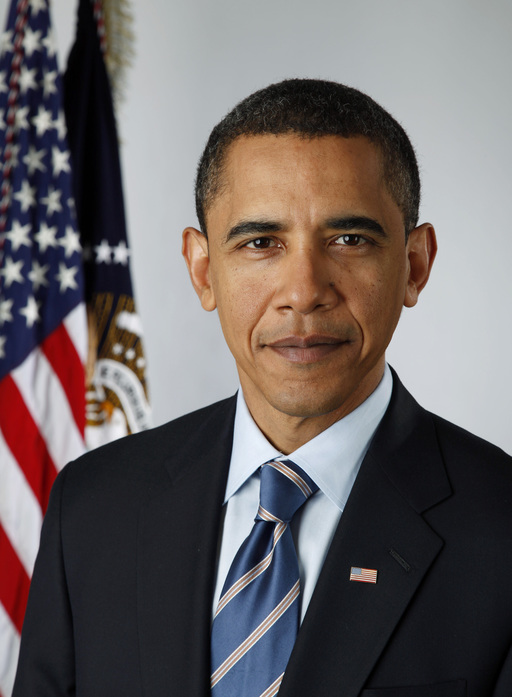
\includegraphics[width=0.9\linewidth]{imgs/obama.jpg}}
							\label{fig:1a}
						\end{subfigure}
						\begin{subfigure}[!ht]{0.48\linewidth}
							\centerline{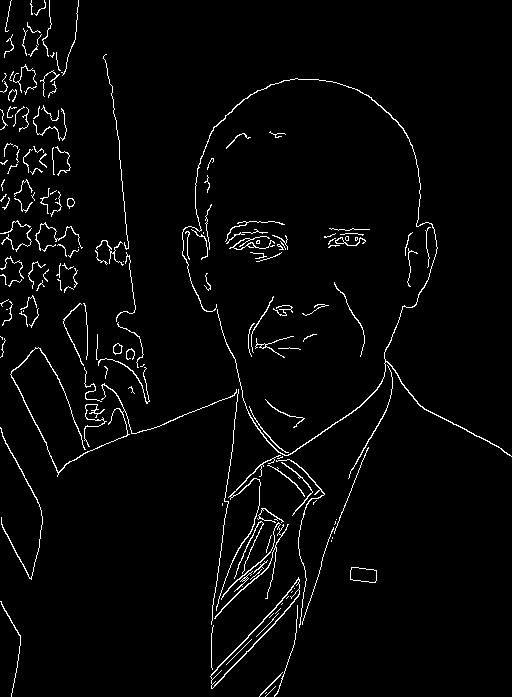
\includegraphics[width=0.9\linewidth]{imgs/obama_edges.jpg}}
							\label{fig:1a}
						\end{subfigure}
						\caption{Example of edge detection}
						\label{fig:1}
					\end{figure*}
					
					\noindent After edge detection, other techniques began to spread for feature extraction. 
					In a paper by Kumar and Kumar Bhatia written in 2014 \cite{kumar2014detailed}, 
					there are some examples of techniques used to extract features. 
					In this paper, the authors present different types of features and then some techniques to extract them. 
					Some of the most important are:

					\begin{itemize}
					
						\item \textbf{Diagonal based feature extraction techniques}:
						
							In this procedure, the image is divided into zones formed by small squares of pixels. 
							In the paper's case, there would be 19 diagonal lines. 
							The value of each pixel in these diagonals is summed to obtain a single sub feature. 
							Then we can extract a feature by averaging the sub features. 
							With this method, we can extract a feature for every zone. 
							Then by averaging the column-wise and row-wise features we can increase their number. 
							
						
						\item \textbf{Fourier descriptors}:
						
							The Fourier transform is commonly used for shape analysis. 
							The transformed coefficient are called the Fourier descriptors.
							These descriptors represent the shape in a frequency domain, with the low frequencies symbolizing the general shape and the high frequencies symbolizing details of the shape. 
							Since the transformation usually generates many parameters, only a subset is considered.
						
						
						\item \textbf{Principal Component Analysis (PCA)}:
						
							This procedure is a mathematical way to convert a set of observations into a set of values of uncorrelated variables. 
							These variables are defined so that the first one has the highest variance, and the components are all orthogonal (independent) from each other. 
							
						\item \textbf{Independent component analysis (ICA)}:
						
							ICA is a statistical technique. 
							It aims to use non-Gaussian random variables to represent multidimensional vectors. 
							The random variables should be as independent as possible. 
						
						\item \textbf{Gabor filter}:
						
							A Gabor is a sinusoid multiplied by a Gaussian, and its response is a convolution operation. 
							This type of filter performs well in both spatial and frequency domains.
						
					\end{itemize}
				
				
				\noindent These were not the only techniques presented in the paper, but since some were more problem-specific (about handwritten character recognition)
				were excluded from the list. These excluded techniques can still be used, but may have worse results or may require some adaptation. 
				The techniques were: Fractal theory techniques, Chain Code Histogram of Character Contour, Finding Intersection/Junction in character, 
				Shadow features of character, Sector approach for feature extraction, Transition feature
				Extraction of distance and angle features, Extraction of occupancy and end-point features, and Zernike moments.\\
				In another paper, written in 2013 by Tian \cite{ping2013review}, there are some other techniques cited that may result useful:
				
				\begin{itemize}
				
					\item \textbf{Colour features}:
						
						Colour is one of the most important features humans can perceive. 
						The features we can extract depend on the colour space, but once it is defined there are some possibilities. 
						A few examples are colour histograms, colour moments and colour coherence vectors. 
						One of the simple and meaningful, according to the authors, is colour moments. 
						The most common colour moments are the mean, the standard deviation and the skewness. 
						
					\item \textbf{Texture features}:
					
						Another very important feature of images is texture. 
						Features involving texture analysis can be extracted from groups of pixels. 
						One of the most common methods is a Gabor filter, which can be used by characterizing the central frequency and the orientation parameters.
				
				\end{itemize}
				
				\begin{figure}[!ht]
					\centerline{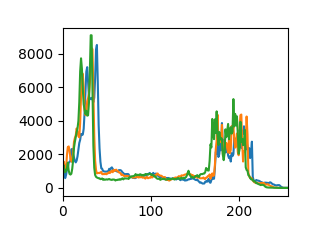
\includegraphics[width=\linewidth]{imgs/obama_histogram.png}}
					\caption{Color histogram of the image used in Figure \ref{fig:1}}
					\label{fig:2}
				\end{figure}
				
				\subsubsection{Deformable shape analysis}
			
					A more sophisticated technique than the ones listed before is shape analysis. Deformable shape analysis, in particular, can be useful to extract features from an image.\\
					In 2005, Felzenszwalb wrote a paper that focuses on representation and detection of deformable shapes~\cite{felzenszwalb2005representation}. For the goal of the experiment proposed here, some deformable shape 
					detection techniques can be useful. \\
					The technique proposed strongly relies on the triangulated polygon representation. This type of representation lets approximate every 2D shape without holes using a representation based on triangles. 
					The author also make use of the properties of chordal graphs and k-trees.\\
					The technique described in this paper falls under the category of deformable template matching. One of the components of the method is the energy function, a function that associates a cost with every 
					possible transformation. The objective is to find the transformation with the lowest possible cost. This component is very flexible, since, depending on the formulation of the energy function, the costs 
					can be tuned even for individual triangles. Moreover, it is also possible to integrate learning techniques to learn deformation parameters.
					Since the possible non-rigid transformations of a template are numerous, this kind of techniques usually require an initialization near to the correct solution, 
					although this is not required for the algorithm presented in this paper. For the implementation of the algorithm itself, a technique called non-serial dynamic programming was the key factor.
					
					\begin{figure}[!ht]
						\centerline{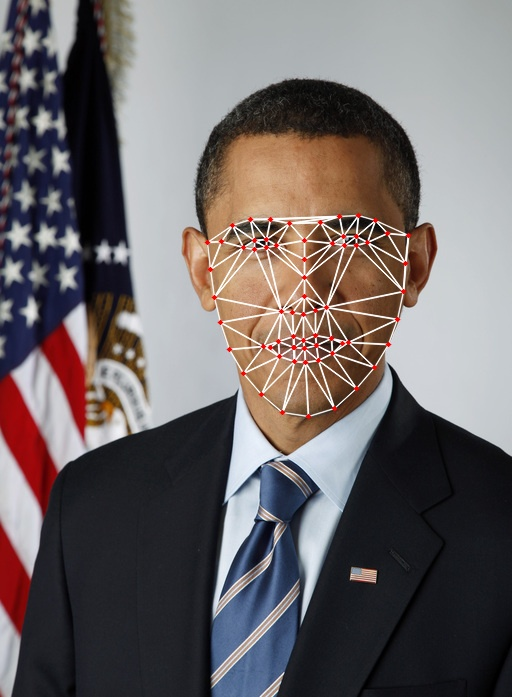
\includegraphics[height=0.4\textheight]{imgs/delaunay.jpg}}
						\caption{Example of Delaunay triangulation, the type of triangulation at the base of Felzenszwalb's paper}
						\label{fig:3}
					\end{figure}
					
				\subsubsection{Machine learning based feature extraction techniques} \label{mlfe}
					
					After the classic techniques, machine learning began to be involved in feature extraction. In particular there are some papers that explain the results achieved with machine learning.\\
					\noindent In 2019, a paper written by Varshni et al. that proposes a method~\cite{varshni2019pneumonia} to classify images using CNNs, trying to understand if a patient 
					has pneumonia or not. After the preprocessing, there is the feature extraction process. For this step, the authors used different pretrained models.
					In this paper's results it is reported that the best model architecture is DenseNet-169.
					
					\noindent In 2019, Guamei et al. wrote a paper about hybrid feature extraction methods to classify brain tumours~\cite{gumaei2019hybrid}. The process described in the paper is divided into three points. The 
					first one is preprocessing, the second is feature extraction and the third is brain tumour classification. The first step is just to rescale the values to the range $[0,1]$. The feature extractor 
					used is the GIST descriptor. The GIST is then combined with a Gabor filter and produces a total of $mxnx4x4$ GIST feature vectors. There is a variant of the GIST descriptor, the 
					PCA-NGIST is a PCA-based normalized GIST feature extraction method. The NGIST is a normalized version of the GIST descriptor, that uses the L2 norm to make the GIST invariant to illumination and shadowing. 
					After this step, the only thing left is the classification of the tumour, which was performed with a RELM classifier. 
					
					\begin{figure*}[!ht]
						\centerline{\includegraphics[width=\linewidth]{imgs/cnn_features.png}}
						\caption{Example of features extracted by a CNN}
						\label{fig:4}
					\end{figure*}	
					
					\noindent In Figure \ref{fig:4} there is an example of feature extracted by a Convolutional Neural Network. 
					
				\subsubsection{Hyperspectral images feature extraction}
					
					Although there exists techniques that can extract features from hyperspectral images, this kind of images are created to capture the entire spectrum. This fact means that these images can capture 
					more information then what the human eye can. The techniques involve, in the majority of the cases, learning of some form, especially in form of neural networks, in particular convolutional recurrent 
					networks, as seen in a paper by Hu et al.~\cite{hu2020spatial} and in a paper by Rasti et al.~\cite{rasti2020feature}. For the reasons just said, it is probably more meaningful to use normal 
					images than these ones.
			
			\subsection{Networks}
			
				\noindent Neural Networks are a powerful instrument in the hands of computer scientists. There exists a lot of different types of artificial neural networks, each with its own peculiarities. In particular, for this 
				experiment the one needed will be, most likely, just convolutional neural networks and siamese neural networks. 
			
				\subsubsection{Convolutional Neural Networks (CNN)}
				
					Convolutional neural networks are not an extremely recent type of neural network, especially if we consider that LeNet-5 was created in 1998. Scientists have dealt with CNNs for some years. Now, as of 2022, 
					CNNs are mostly used to deal with images.\\
					In 2017, Wu wrote a paper that had the purpose to serve as an introduction to CNNs~\cite{wu2017introduction}. These networks use mostly three kind of layers: Dense layers (which are fully connected layers), 
					Convolutional layers and Pooling layers. In the following, there will be a short description of each kind of layer. 
					\begin{itemize}
						
						\item \textbf{Dense layer}:\\
							The dense layer is not peculiar of CNNs, in fact it is found in almost all types of neural networks. It consists of a set of neurons that are connected with every neuron of the previous 
							layer. Dense layers are usually used towards the end of the network.
						
						\item \textbf{Convolutional layer}:\\
							Convolutional layers just compute a convolution operation. This helps reducing the input size and extract meaningful features from the image taken as input. These layers are usually used 
							in the first layers of the neural network.
						
						\item \textbf{Pooling layers}:\\
							Pooling layers downsample the image to reducing the number of parameters needed. These layers are usually alternated with the convolution layers, so are used at the beginning of a neural network.
							
					\end{itemize}
					
					\noindent The applications of deep learning and CNNs are numerous. As shown previously, there are some CNNs used in image classification with the objective to identify diseases. The typical example is 
					the pneumonia detection. Another possibility is to use CNNs in segmentation or self driving cars, as stated in \cite{alzubaidi2021review} by Alzubaidi et al.
			
					\begin{figure}[!ht]
						\centerline{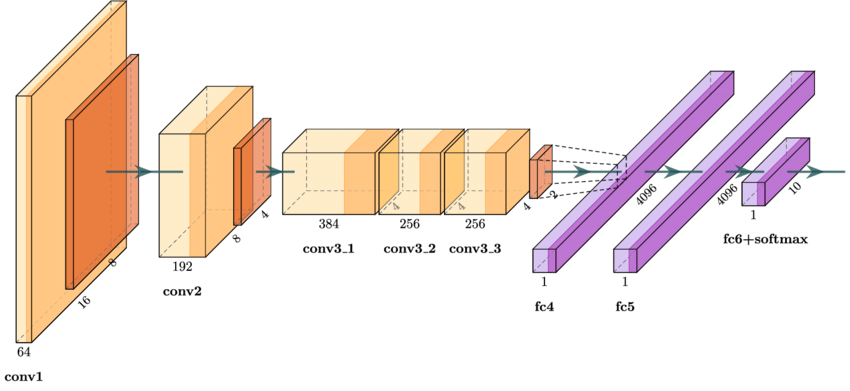
\includegraphics[width=\linewidth]{imgs/cnn_architecture.png}}
						\caption{Example of CNN architecture. In particular, this image represents AlexNet's architecture}
						\label{fig:5}
					\end{figure}
					
					\noindent In figure \ref{fig:5} there is an example of the architecture of a CNN, in particular AlexNet is the CNN chosen for this example. 
					
				\subsubsection{Siamese Neural Networks}

					Siamese neural networks, also called twin networks, are a more recent advance in computer science. These neural networks have a different structure from convolutional neural networks. The 
					structure of siamese neural networks is peculiar. In fact, there are two identical networks, called embedding networks, that process different inputs and, after that, 
					they merge in a single layer that measures the similarity between 
					the two outputs of the two networks. The siamese neural networks have a different application compared to CNNs, in fact twin networks are mainly used to measure similarity of two objects. 
					In the case of this paper, the siamese neural networks are used for image matching. This is not the first time that siamese networks are used for image matching, as shown in a paper written in 2016 by 
					Melekhov et al.~\cite{melekhov2016siamese}, but with a little difference in the objective of the matching. The objective of the paper was to learn a general similarity for image retrieval, while on the case of this 
					paper, the objective is to find a similarity measure with a prototype. 
					
					\begin{figure}[!ht]
						\centerline{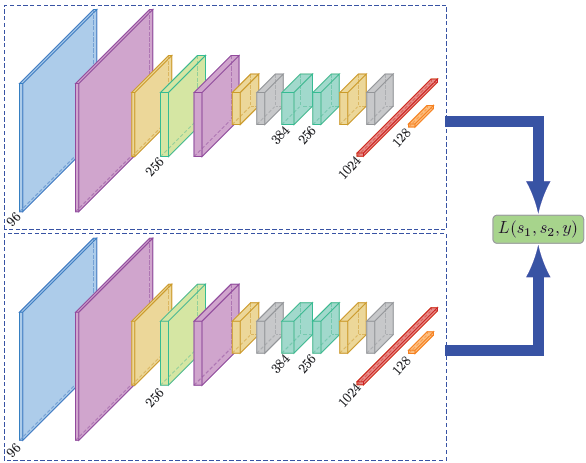
\includegraphics[width=\linewidth]{imgs/siamese_architecture.png}}
						\caption{Example of a Siamese Network architecture.}
						\label{fig:6}
					\end{figure}
					
					\noindent In Figure \ref{fig:6} there is an example of a Siamese Neural Network, in particular the two embeddings are convolutional neural networks. 
			
			\subsection{Similarity judgments}
				
				\noindent In the past there have been some works regarding image similarity, like for example the one presented by Appalaraju and Chaoji in 2017~\cite{appalaraju2017image}. In this work they explore the possibility to 
				find a similarity measure for image retrieval. To achieve this goal, they implemented a siamese neural network that uses two identical multi-scale CNNs that share weights. The ouput of the 
				network is binary, being $1$ the label to predict in case of negative examples and $0$ the label to predict in case of positive example. The loss function used in this work is a contrastive loss. This paper 
				then proceeds to explain a technique called Online Pair Mining Strategy (OPMS), inspired by curriculum learning, that helps reducing the training time. \\
				This is not the only work that uses neural networks to learn similarity, in fact there are also other application fields for similarity study. One of them is healthcare, as shown in a paper by Suo et al., written in 
				2017, that introduces a model used to make personalized prediction of diseases for patients, basing the prediction on a similarity related method, learned using CNNs~\cite{8217759}. In this paper, before 
				learning the actual similarity measure, the authors processed the input through a CNN and performed a step they call ``Time fusion''. This step let them incorporate the time information and 
				weight differently eventual symptoms based on their temporal distance from the first appearance of the disease. Only after this step the authors proceeded to learn a similarity metric, basing the learning 
				on CNNs.\\
				Another paper, written by Chopra et al. in 2005, used a method similar to the one written by Appalaraju. In this work, the authors used a siamese architecture to learn a similarity metric and applied it 
				in the field of face verification~\cite{chopra2005learning}.\\
				More interestingly, there are also other papers, in particular a paper by Attarian et al. written in 2020 uses $VGG16$. This paper's goal is to use this CNN to predict human similarity 
				judgments~\cite{attarian2020transforming}. Using $VGG16$, the authors were able to achieve good results, with over 90\% in validation accuracy.
				
	\section{Data Collection}

		\subsection{Image collection}
			
			\noindent Since the proposed experiment uses neural networks, there is the need to have a lot of data. In this particular case, there is the need to gather many images. There are some image dataset, intended for computer 
			vision\footnote{\url{https://imerit.net/blog/22-free-image-datasets-for-computer-vision-all-pbm/}}, that could help. Some of the dataset reported there are quite famous, like ImageNet or Google's Open Images. The 
			best for this kind of work, though, is to have a dataset of which every image is part of the same ``macro-category'', like for example a dataset made of images of birds. Even though this is the ideal case,
			most of the dataset that are used for computer vision contain more than one single category. For example, ImageNet, which is one of the most famous image datasets, contains more than 1 million images that are divided 
			into 1000 classes. Generally, it is possible to use these datasets, which have different macro categories, by filtering the input images based on the macro category the experiment uses.
		
		\subsection{Rating based method for typicality values\label{sec:typval}}
			
			\noindent In this experiment, typicality judgments play a crucial role. To gather enough data about the perceived typicality of images, a form is necessary. This survey should be structured in a way that presents an 
			image at a time to the subject that is taking the survey and asks to rate the typicality of the object portrayed in the image, possibly in a given range. If that is the case, a range between $1$ and $10$ 
			could be the best decision since people are quite used to rate in this range. Once there are enough results, the various rates should be averaged so that there is a single measure that takes into 
			account every rate taken from the survey. The number of people that should participate in the experiment should be high enough to be a meaningful statistical group.
			
		\subsection{Typicality ranking methods for typicality values}
		
			\noindent Another possibility for collecting typicality values is the typicality ranking. With this method the researcher asks subjects to rank a set of objects based on their typicality. After doing so 
			and collecting the data, the researcher should infer the typicality values based on the ranking. The ranking, as the rating described in \ref{sec:typval}, cannot be performed on all images of the dataset, 
			so it's necessary to split the ranking and rank the images in different forms and then use the informations coming from different subjects and infer the informations about typicality from these answers.
			
		\subsection{Possible alternative to typicality values\label{sec:patv}}
		
			\noindent Another possibility to gather data, it is to ask people to list a certain number of objects or all the objects the subjects can think about of the decided category. For example, let us assume the macro category decided 
			is ``birds''. It is possible to collect enough data by asking people to list the first few examples of birds, using a predefined number. Moreover, it is possible to use a variant of this procedure and ask people 
			to list all the examples of birds that they can think of. These two variants of the same data collection approach are both possible and come with some advantages and disadvantages when compared to the other 
			method described in \ref{sec:typval}. 
			
		\subsection{Test of the alternative data collection method}
	
			\noindent To test the method of data collection described in \ref{sec:patv}, I collected the results of a small survey in which there were 10 questions, each asking to give the name of a bird. The number of 
			people that answered is not big enough to be a statistically relevant group, since the number of the answers is only $14$.
	
		\begin{figure*}
			\centerline{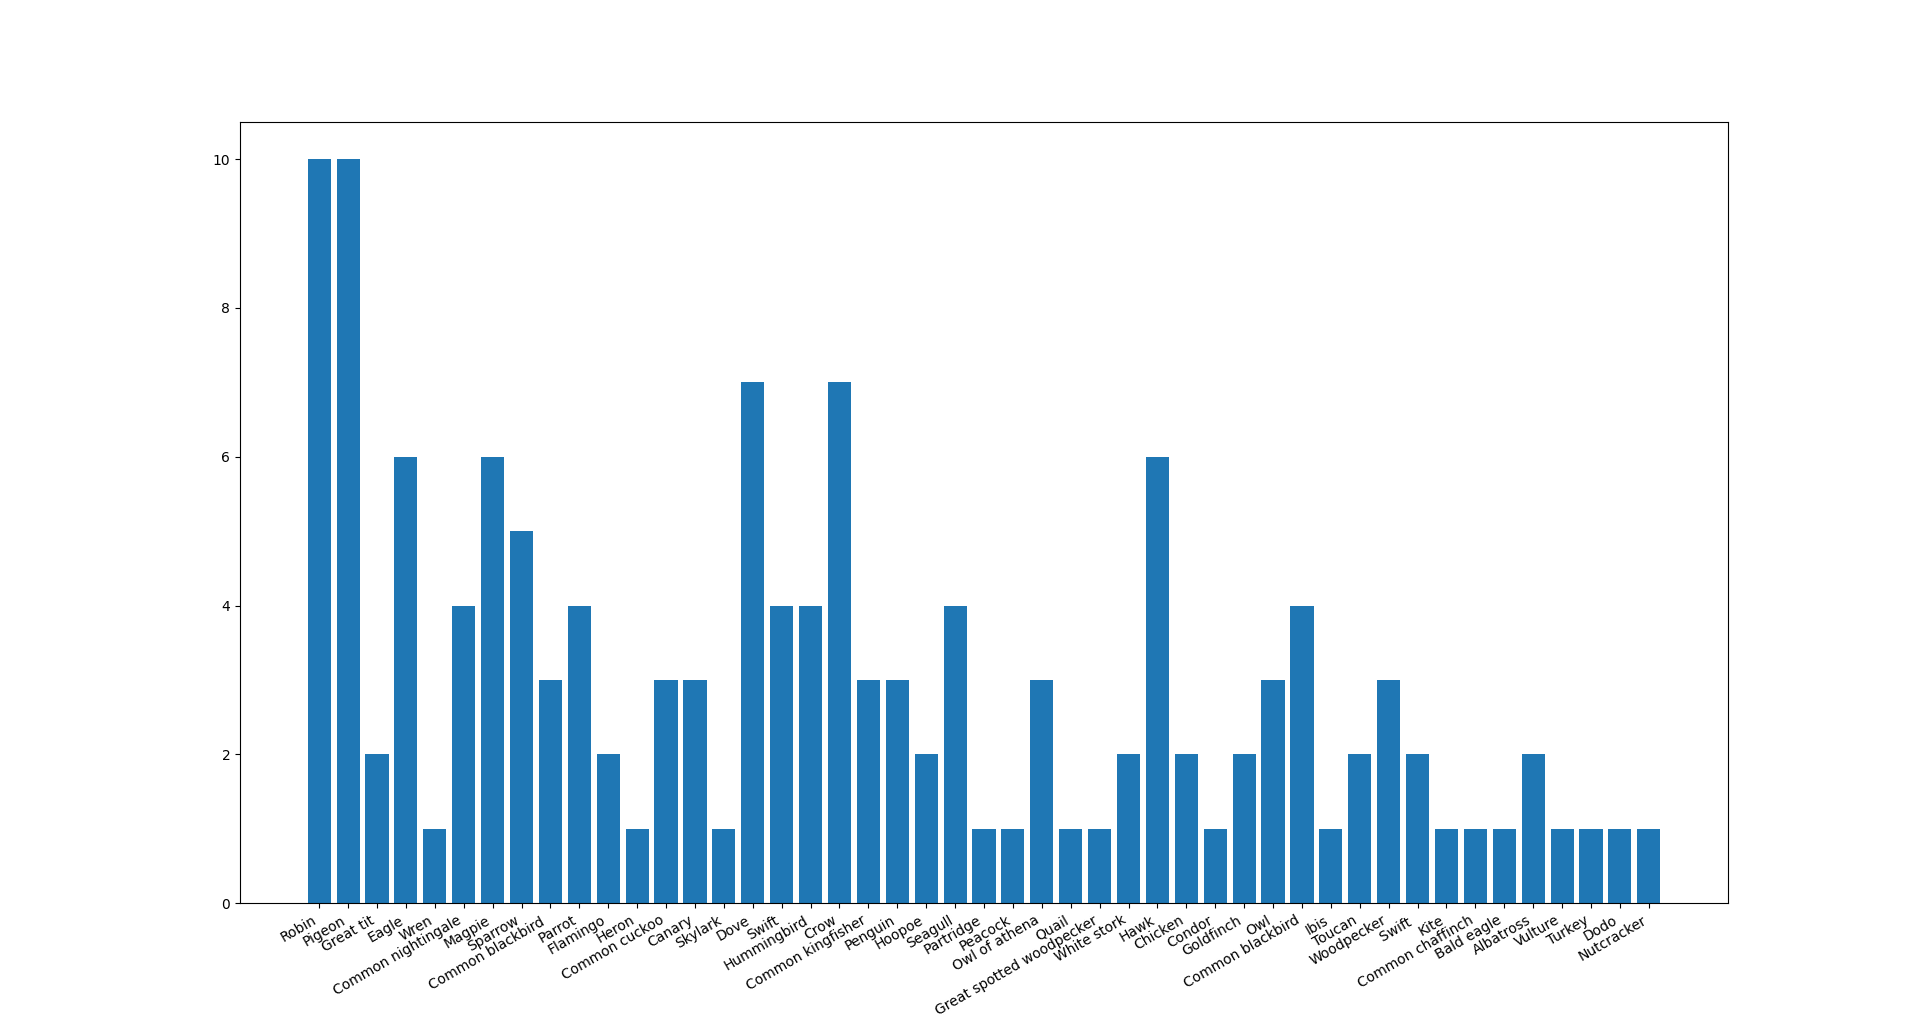
\includegraphics[width=\linewidth]{imgs/survey_hist.png}}
			\caption{Results of the survey}
			\label{fig:7}
		\end{figure*}
		
		\noindent In Figure \ref{fig:7} there are the results of the survey. Even though the number of answers was not very big, some problems still emerged.
		\begin{itemize}
		
			\item \textbf{Off-topic answers or blank answers}:
				
				In this case, one of the answers had to be deleted from the answers, since the cited example was not part of the category decided for the survey. In particular, the survey asked for examples of birds, 
				while one of the answers was a mammal. This fact highlights a problem bound to the number of examples the user knows or can think of. In this example, the survey asked for $10$ names of birds,
				which I thought was a reasonable number, but probably some of the subjects that took part to this survey could not think of a $10^{th}$ name, so just put a name of another animal. The solution 
				to this problem is to apply some data cleaning to the answers to filter the examples that, eventually, are in the answers but not part of the given category. An analogue approach can be applied if the 
				subject leaves the answer blank for the same reason.
			
			\item \textbf{Capitalization of examples}:
			
				This problem is simpler than the previous one to solve, since it just involves the capitalization of the answers. If the survey starts accounting numerous results, it becomes difficult to 
				compute the number of times that a particular example appears in the answers, so, most likely, there will be some automated scripts that compute all the needed statistics. This could be a problem since 
				in most of the programming languages, if not all, words like ``Robin'' and ``robin'' are considered different based on the capitalization. This problem is easily solvable by lowercasing all the 
				answers.
				
			\item \textbf{Typos of examples}:
				
				This problem can be quite challenging to solve. In fact, subjects could make some mistakes when typing the answers, so for example a word like ``robin'' can become ``ribin'' or ``tobin'' for example. 
				Moreover, if more than one letter is wrong, some results like ``rivim'' instead of ``robin'' are possible, especially if the subjects compile the form via mobile devices. To solve this issue, 
				it is possible to use some distance between strings, like for example the Levenshtein distance, which is used to find the distance between two strings. Although this could be a solution,
				it is not guaranteed that the result is correct, so these results should always be checked again to prove they are correct and, most importantly, coherent with the category the survey is based on.
				
			\item \textbf{Different specificity levels}:
			
				This problem is very difficult to overcome. There is an example in the histogram reported as results. In the histogram, in fact, it is possible to note that there are both the ``eagle'' and 
				the ``bald eagle'' labels. This means that different subjects can answer with different levels of specificity, since the ``eagle'' label is more general than its counterpart ``bald eagle''. 
				This problem is presented also in an inter-species context, for example the ``Common kingfisher'' represents a single specie, representative of the ``kingfisher'' genus, while, for example, 
				``Flamingo'' represents a family, of which some examples are the greater flamingo and the lesser flamingo, along with other species as well. 
				Even though the problem is very clear, it is not very clear what to do in this case. A possibility is to decide that, in the case of the presented survey, 
				the ``bald eagle'' label should be incorporated in the ``eagle'' 
				label, making sure that all the instances of the most specific one are accounted as instances of the more general one. Another possibility is to keep both of the labels, so that the results of 
				the survey are unaltered. Lastly, it is possible to assume that every label that identifies a group more general than a single specie, like a family or a whole order is referred to the most 
				common specie of that family or order. The only way to know exactly which of these possibilities performs better is conducting some experiments and compare the obtained results.
		
		\end{itemize}
		
			\noindent Even with all these problems, the survey works quite well, since also with a few answers the results show that most of the subjects had mentioned the most common birds, like pigeons, while the 
			less common ones, like for examples peacocks, are mentioned fewer times. The results of this particular survey show that, a part for some examples, most of the birds appear only a few times. Although there 
			are some examples that are most likely outliers even with large numbers of subjects taking the survey, like ``Dodo'', some other examples, like ``Swift'' or ``Common blackbird'', 
			are likely to be more typical with a larger number of people taking the survey.\\
			The goal of the survey is to infer a measure of typicality based on how often a certain example appears in the results of the answers, and the result, at first glance, seems to be achieved. Although only 
			a test can prove this, it is very likely that with a larger group of subjects taking the survey, the results will differ more than with a small number of subjects. 
		
		\subsection{Considerations about the survey\lable{sec:cas}}
		
			\subsubsection{Considerations}
				\noindent The first two presented methods have a quite similar concept behind them. Although it is still a matter of discussion which one is more reliable, especially in children, as seen in \cite{maridaki1997rating} 
				and \cite{10.1371/journal.pone.0157936}, both these methods have been used to collect typicality informations. The main difference in these two methods is that the first one, which is based on 
				ratings, the researchers may have biased data since it is possible that seeing a picture of an example of the category the subject can be biased. On the other hand, the other method does not present 
				this kind of bias, but presents a higher difficulty on in extracting the typicality values. \\
				The alternative possible proposed method, can show a lower bias than the bias of the rating method since no images influence the subject's ratings. Moreover, it is easier to infer a typicality value 
				than in the ranking method, since a higher position on the list corresponds to a higher typicality. 
				Another positive aspect of this method is that if a person did not think of a particular example, it won't appear on the ratings. This fact can help identifying the real typicality 
				without the possible bias introduced by presenting to a subject an image of an example that did not come to mind. 

			\subsubsection{Limitations and negative aspects}
			
				The biggest problematic related to the first two methods presented, which are the rating and the ranking systems, is that it is not feasible to either rate or rank every example in the whole 
				dataset, since it must have many images. In fact, it is very likely that a subject that has to rate or rank many examples will be tired after a certain number of images, polluting the results of the survey.
				The possible solution to this problem, is to give the subjects a subset of images to rate or rank. In this way, the collected data are most likely more reliable than the ones collected on all the dataset, 
				so it is more accurate the final result. \\
				Regarding only the typicality rating system, there is another problem. As hinted in previously, there is the possibility that this procedure leads to biased data. That is true because the form 
				created to collect the data, presents an example of an object that the subjects may not have thought of, and presenting the image, it may be possible that the subject gives a biased answer since 
				the image could have influenced the subject's judgement. For example, let us assume that the category chosen for the experiments is ``bird''. If a person is presented and image of a swan, 
				or a duck, and is asked to rate its typicality, most likely will rate it in the higher part of the scale, while if asked to list a certain number of birds it is more likely that it is not 
				present than that it is present.\\
				Talking about the ranking system, also this method can present biased data, since also this method presents the images, even if the bias is probably lower than the one that could result with the ranking system. 
				The major problem, with this method, is that the researcher must also design an algorithm to infer the typicality values from the rankings. This is a very difficult algorithm to design, since the rankings must 
				find a mapping to a scale.\\
				The alternative possibility described, can result in a lower bias since no images influence the subject's judgments. Recalling the previous example, in fact, if the subject did not think of 
				ducks and swans in the category ``bird'', these examples will not appear on the list. Although this technique presents a lower bias, it results in a great difficulty in prototype construction.
			
			\subsubsection{Considerations on how to choose}
				In order to give the proper weight to both the pros and cons and decide which is the best, the best decision is asking for help to a psychologist or a neuroscientist so that both pros and cons of the two 
				methods have the right weight and it is easier to decide which one is more convenient.
				As alternative, it is possible to try both the methods and see which one gives better results. In this way, both the possibilities will be used and there is the possibility to see which one is better in 
				terms of performance. 
			
	\section{Feature Extraction\label{sec:fe}}

		\noindent While collecting the needed data with the survey, it is possible to begin the feature extraction procedure. There are various possibilities for this step, as shown in Section \ref{sec:bfe}, which is
		the section dedicated to feature extraction background. 
		It could be interesting to test both classical and machine learning methods, to measure which one is the most efficient. Since feature extraction has already been described in the paper, this section will 
		present a discussion about the results of the presented methods' results. The main difference between the classical and the machine learning feature extraction techniques is human interpretability. 
		In fact, for classical feature extraction techniques, humans have no difficulty in interpreting the result of the process. For example, in edge extraction, humans have no difficulty in recognizing if the 
		edge extracted is correct or not seeing the original image. For example, in Figure \ref{fig:1} no one has any problem to recognize that the figure on the right is the one that draws the edges of the figure on the left, 
		while in Figure \ref{fig:4} there is no clear correlation between the feature and what it means in the image itself.
		Moreover, classical and machine learning features can give different weights to different features. 
		In fact, classical methods rely mostly on features that humans consider important, on the basis of general experience about the world, but also based on the way our brain works. An empirical confirmation of this fact 
		can be that if a person asks to another person to describe, for example, a common kingfisher, the person that should describe the bird will, most likely, start describing the dimension, the shape, and only 
		later the colour. Machine learning techniques, on the other hand, could give a very high importance to the fact that the bird is mainly blue and red, if they have access to the colour information. Due to the fact that 
		the blue colour is not very present in nature, the blue and red couple of colours can be highly characteristic of the common kingfisher, even if humans give, unconsciously and innately, more importance to 
		shape-related features.	\\
		If the data collection method chosen is the one that asks people to list the objects of the category, the feature extraction can happen in two possible ways. The first way is to use the data collected for 
		typicality judgments and collect also images of the examples that appear in the results. After collecting enough images, the feature extraction process can proceed as described earlier and use either  
		classical or machine-learning-based feature extraction methods. Although this is a possibility, there could be an alternative. The alternative seems interesting because it can be adapted to rely only on features 
		that humans identify as important. To do so, the survey should include a question that asks the subjects to list all the characteristics that the objects of the given macro category have in common. In this case, 
		the features are not strictly extracted by the dataset, but are listed by the subjects that take part in the survey. By doing so, the experiment takes into account, in the prototype, only the features that 
		human have listed, so only the features that are considered important by humans themselves. Although it is theoretically possible, this procedure will result in numerous complication in prototype construction. 
		

	\section{Prototype construction}

		\noindent The construction of the prototype is one of the most delicate parts of the experiments. How this phase works depends heavily on what method was used for feature extraction. 
		
		\subsection{After classical feature extraction techniques\label{sec:cfet}}
		
			\noindent In case classical feature extraction techniques were used, the goal of this activity is to build an image that presents in itself a ``prototype'' of the object. For example, a prototype of a bird, could be 
			an imaginary bird with a shape that it is obtained with a weighted average of the shapes of all the birds in the image. For example, since birds like sparrows and swifts are perceived as more 
			typical than ostriches and penguins the prototype should resemble more swifts and sparrows than ostriches and penguins. To do so, the key factor is performing numerous analyses on various 
			different subjects, until there are enough data to have a statistical value. 
			
			\begin{figure*}[!t]
				\centering
				\begin{subfigure}[!t]{0.48\linewidth}
					\centerline{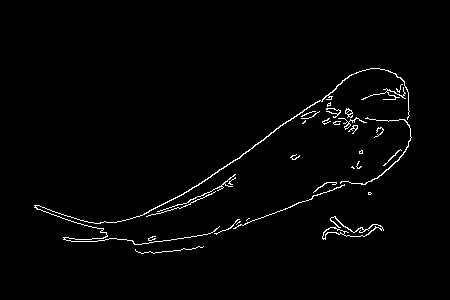
\includegraphics[width=0.9\linewidth]{imgs/swallow_edges.jpg}}
				\end{subfigure}
				\begin{subfigure}[!t]{0.48\linewidth}
					\centerline{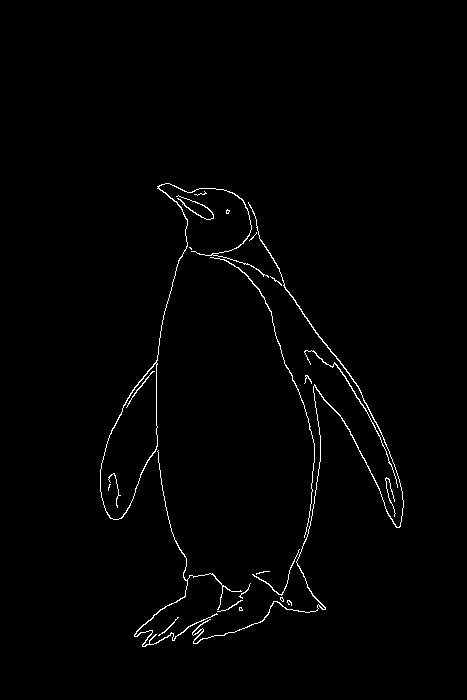
\includegraphics[height=0.4\textheight]{imgs/penguin_edges.jpg}}
				\end{subfigure}
				\caption{Edge extraction of swift and penguin}
				\label{fig:8}
			\end{figure*}
		
		\noindent In Figure \ref{fig:8} there is an example of the edges of two different birds. Although both of the original 
		subjects are birds, one is much more typical than the other one. In this case, the prototype should try to match more the swift edge than the penguin edge. A way to do so could make use deformable 
		template matching. Matching a shape with a template could be useful to find a weighted average between the two shapes. In this way, the resulting shape takes into account both the original edges while 
		giving priority to the one more typical.
		This procedure should be applied for both shape features and colour features, so that all the features that can be extracted from the prototype image resemble the weighted average of all the feature from 
		the original images. 

		\subsection{After machine learning feature extraction techniques\label{sec:mlfet}}
		
			\noindent In case machine learning feature extraction techniques were used, it is conceptually and practically easier to compute the average features. In fact, the features extracted by machine learning techniques are 
			in the form of arrays of numbers, so to compute the prototype of the image in this form it is enough to take the weighted average of the vectors. The weights should be taken according to the perceived typicality 
			of the category example, which is the average of the measures collected with the survey.
			
		\subsection{After the alternative data collection method}
		
			\noindent If the method used for data collection is the one described in Section \ref{sec:patv}, the feature extraction can take two different paths. One of these two paths leads to collecting 
			several images and applying one of the classical or machine learning-based feature extraction techniques. In this case, the prototype construction follows the guidelines given in Sections \ref{sec:cfet} and \ref{sec:mlfet}.
			In case the features are not extracted directly from images, but from answers on the survey, the process is more complex. In particular, the construction should generate a prototype from 
			scratch based on the indications on the survey. The importance of every feature can be deduced by how many subjects mention it in their description. The result should be in the form of an image. 
			As mentioned when talking about the prototype construction after classical feature extraction methods, the image generated by this process should take into account more the features listed more 
			times in the survey, since they would be features that more people identify as important. In a way similar to the one that is described earlier, the prototype must be built in the form of an image. 
			The challenge that this procedure presents, though, it is different than the one presented by the other method, since the image in this case has to be built from scratch, having only the indications of 
			those who participated to the survey. To make the prototype construction easier, there is the possibility to build from scratch a prototype for every answer of the survey and then merge them all in one 
			single image, taking into account the different contributions based on how frequently some characteristics are mentioned. In this way, even though the procedure demands the construction of more than one 
			image, the final prototype is obtained by summing all the single images using a weighted sum.
		 
		
		\subsection{Considerations about prototype construction\label{sec:cpc}}
		
			\noindent The prototype depends on the feature extraction technique that was used. As discussed in Section \ref{sec:fe}, the key difference is human interpretability. In fact, building a prototype using the 
			classical feature extraction methods, results in an image that can be seen and interpreted. Using a prototype generated with machine learning feature extraction techniques results in an array 
			of numerical values, that are not easily interpretable. As of 2022, there has been some research on the topic of interpretability and explainability of machine learning, like for example 
			a work by Carvalho written in 2019~\cite{electronics8080832}, 
			but the field is still growing, also given the interest deriving from the AI-Act, the proposition of the European Union in the field of artificial intelligence. In particular, there is a document of 
			the act\footnote{\url{https://eur-lex.europa.eu/resource.html?uri=cellar:e0649735-a372-11eb-9585-01aa75ed71a1.0001.02/DOC_1&format=PDF}} that states that there will be some requirements in terms of 
			transparency and interpretability for machine learning systems that are considered high-risk AI. The growing interest produced some results, but still they are not enough to easily interpret machine learning 
			features.\\
			Most likely, in the future will be possible to look at the features extracted by a neural network and comprehend their meaning. When this will be possible, independently of the feature extraction techniques 
			used, the human interpretability will be possible, and with that in mind it would be probably more convenient to extract the features using neural networks. The reason behind this consideration is 
			that although the training of a neural network can be expensive in computational terms, the evaluation of an input on a trained network it is not very computationally demanding. On the other side, algorithms 
			like the triangulation always have the same demand, that is lower than the demand of training a neural network, but surely higher than the demand of evaluating a single input on a convolutional neural network. 
			Moreover, considering the possibility to use transfer learning techniques, the training can become a fine-tuning or a domain adaptation problem, which means the computational load is lighter. Considering that 
			the fact that the training is a demanding task to be performed only once and that other algorithms may be less demanding but must be run multiple times, it is probably more convenient to train a neural 
			network. Moreover, not only the feature extraction process is convenient, but also the prototype construction itself is more convenient if the features are in the form of numerical parameters, since it is 
			enough to perform a weighted average, a simpler operation if confronted with the construction of a new image that should take into account features of numerous other images.
			Moreover, scientists will be presented a tough challenge, since the construction of an image using the average of other images is not an easy task. In this task there are in particular two problems. The first 
			one is that there is no clear algorithm to average two different images as it is requested in this paper, 
			and it is even more difficult to compute a weighted average. In fact, the in Figure \ref{fig:8}, it is difficult to even imagine what the result of this weighted average should be. 
			
			\begin{figure*}[!t]
				\centering
				\begin{subfigure}[!t]{0.48\linewidth}
					\centerline{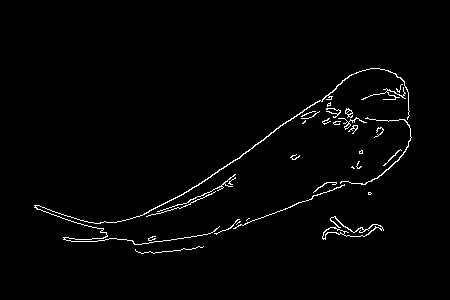
\includegraphics[width=0.9\linewidth]{imgs/swallow_edges.jpg}}
				\end{subfigure}
				\begin{subfigure}[!t]{0.48\linewidth}
					\centerline{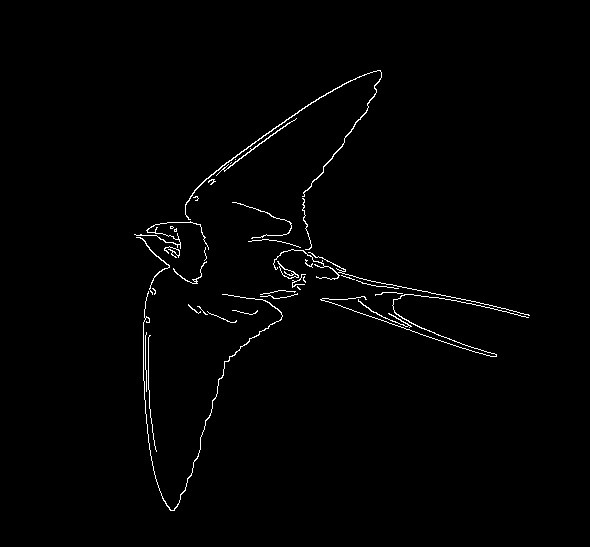
\includegraphics[height=0.4\textheight]{imgs/swallow_2_edges.jpg}}
				\end{subfigure}
				\caption{Edge extraction of different swifts}
				\label{fig:9}
			\end{figure*}
			
			\noindent The second problem is concerning the weight of the image portrays the same example in different positions. Talking about birds, there is an example in Figure \ref{fig:9}. In this case, it is not clear 
			how much should the first image weigh compared to the second one, since they portray the same species of bird in different situations. As said before, there is no algorithm that can average the two images in the 
			way required by this paper, but in this case, most likely, the result would be a mix of two images that would not have much sense, since the swift is in different position, in one it is perched while in the other 
			image is flying. So, to work with this type of approach, an algorithm that computes the average of the two images should be implemented.\\
			If the data are obtained with the alternative data collection method proposed, the construction can take two different paths. For the first, which is collecting images based on the survey's answers, the 
			considerations done earlier remain valid, since in the end the feature extraction happens on an image dataset. There is another possibility, though, that is more difficult to implement. In this case, the 
			prototype is built from scratch, using the informations that the subjects gave in the survey. This method theoretically is more accurate than the others, since it can take into account only features 
			that the people answering have in mind. On the other hand, people could not list some features that they consider important because they take them for granted. An example is the presence of the beak in birds. 
			Most likely, the vast majority of people imagine a bird with a beak, but take for granted the presence of the beak, so it is unlikely that it is listed in the features. On the contrary, it is very likely that 
			most people will list, for example, wings in the features that a bird should have, without specifying which type of wings. 
			
			 \begin{figure*}
				\centering
				\begin{subfigure}{0.48\textwidth}
					\centering
					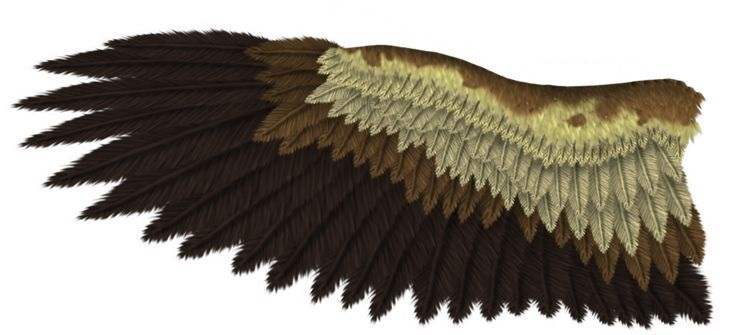
\includegraphics[width=\textwidth]{imgs/eagle_wing.jpg}
					\caption{Eagle wing}    
					\label{fig:9a}
				\end{subfigure}
				\hfill
				\begin{subfigure}{0.48\textwidth}  
					\centering 
					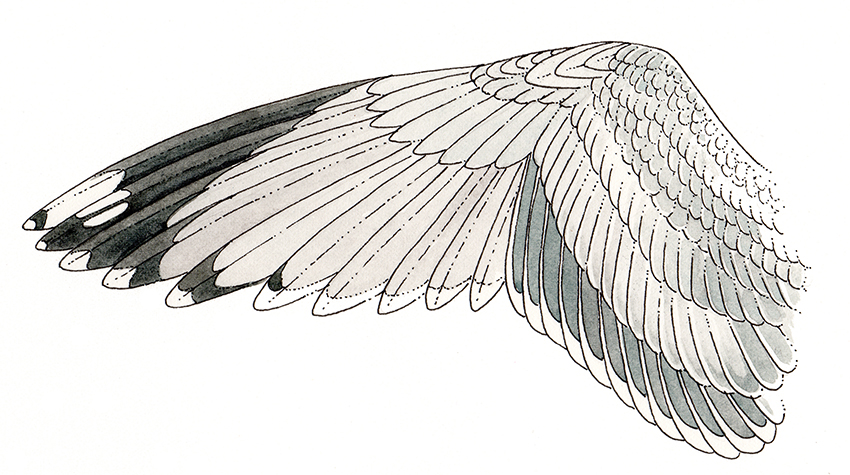
\includegraphics[width=\textwidth]{imgs/seagull_wing.jpg}
					\caption{Seagull wing}
					%\label{fig:9b}
				\end{subfigure}
				\vskip\baselineskip
				\begin{subfigure}{0.48\textwidth}   
					\centering 
					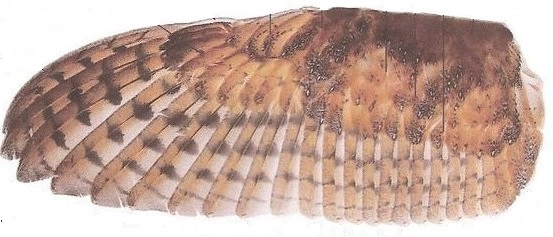
\includegraphics[width=\textwidth]{imgs/owl_wing.jpg}
					\caption{Owl wing}
					%\label{fig:9c}
				\end{subfigure}
				\hfill
				\begin{subfigure}{0.48\textwidth}   
					\centering 
					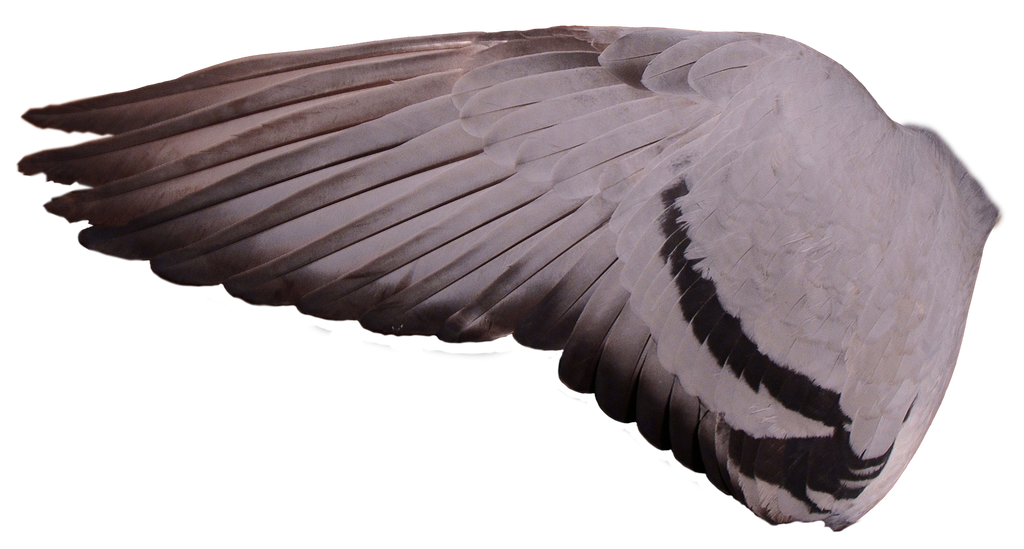
\includegraphics[width=\textwidth]{imgs/pigeon_wing.png}
					\caption{Pigeon wing}
					%\label{fig:9d}
				\end{subfigure}
				\caption{Different types of wings of birds}
				\label{fig:10}
			\end{figure*}

			\noindent In Figure \ref{fig:10} it is possible to see some wings of different birds. As shown by the images on the picture, the wings of different birds tend to be different, even if some have more 
			differences than others. For example, the eagle's wing and the owl's wing are more similar to each other than to the others, since both of them are raptors. Even though these two birds are part of 
			the same order of birds, their wings differ from one another since the owl has a feather conformation that make sure that there is almost no sound when the bird is flying, while the eagle's wings 
			help the bird fly with the minimum effort. The seagull and the pigeon wings, on the other hand, differ a lot from the wings of the two raptors, since they are part of another family, so they adapted 
			the shape of the wings for other goals. These considerations lead to understanding that even if a person, interviewed for the survey, tells that having wings it is a common characteristic of birds, 
			it is important to understand what type of wings the subject is talking about. Moreover, the characteristics should be as precise as possible in terms of descriptive quality, since the prototype, a 
			key factor of this work, relies on the description made by who is taking the survey. To be as precise as possible, the best way to proceed is to build the prototype with the subject that described it 
			or asking the subjects to draw a sketch of the prototype. To draw the prototypes with the subject present in that moment is something that it is not possible if the number of answers is large 
			enough to be statistically relevant, while may be the case that asking people to draw a sketch and applying some post-processing to the image is easier than building all images from scratch and also 
			reduces the bias to which the data are exposed. In this case, the bias would originate from who builds the prototype, because this person can have its own idea of prototype of the given category and 
			interpret the indications in a certain way that does not reflect completely the original subject's idea. 

	\section{Similarity learning}
	
		\noindent The similarity learning is the core part of the experiment. In this experiment, the similarity learning is done through a siamese neural network but, as the previous steps, depends on the 
		feature extraction techniques used. 
		
		\subsection{Using classical feature extraction techniques\label{sec:slcfet}}
		
			\noindent If the feature extraction process happened with classical techniques, after the prototype building step the result is an image. This means that the two embedding networks must be able to process 
			images. Most likely the best choice, in this case, is to implement two CNNs as embedding networks and merge them in a single fully connected network for the siamese similarity learning. 
			In this case, the siamese network would be fed the prototype image and an image from the dataset. The goal of this kind of prediction is to learn a similarity metric with some annotated values. 
			After learning the similarity metric, the network will be able to measure the similarity of the prototype image and any other image fed in the other embedding network. By doing so and retrieving various 
			measurements the couple of values \textit{perceived typicality - similarity measure} could reveal some interesting patterns.
		
		\subsection{Using machine learning feature extraction techniques\label{sec:slmlfet}}
		
			\noindent If the feature extraction process involved neural networks, after the prototype building step the result is not any more an image but it is a vector of values. This implies that there is no need to 
			use a convolutional neural network as embedding, but it is enough to have some fully connected layers that will be merged in a single fully connected network for the similarity learning. The rest of the procedure 
			is similar, since the siamese network will still be fed the features of the prototype and the features of an image of the dataset. As in the previous case, the goal of this kind of prediction is to learn 
			a similarity metric using annotated values. After learning the metric, the network will be able to measure the similarity of the prototype and any other image. 
			As in the previous point, the couple of values \textit{perceived typicality - similarity measure} could reveal some interesting patterns.
			
		\subsection{Using the alternative data collection method}
		
			\noindent In case the data collection happened with the alternative method, the similarity learning happens with a siamese neural network which structure depends on the feature extraction method described. The 
			results, in fact, can be different. If the data collection is made by looking for images of the cited examples, the feature extraction process can follow two routes: the classical one and the machine learning 
			one. In both cases, the similarity learning follows the descriptions in \ref{sec:slcfet} and \ref{sec:slmlfet} respectively, since the resulting prototypes are images. In case the feature extraction did not happen through 
			the collection of images but creating an image following the features listed by the subjects of the survey, the similarity learning still happens with a siamese neural network, but with some differences. In fact 
			the image resulting from this process will have less features than an image retrieved online, because it is created from scratch using the indications of people that took the survey. Involving humans in 
			the feature extraction process, it is possible that the extracted features will not involve colour features, since the colour feature is dependant on the example of the class. If we consider the class ``bird'' as
			example, the colour that people associate with birds is dependent on the species of the considered bird. If the example taken into consideration is the swift, the colour associated with this bird are, most likely, 
			black and white, while for example if the person thinks about a sparrow, the colour thought about are mostly some brown shades. In order to reduce as much as possible colour features, the images fed to 
			the siamese neural network should be preprocessed. Transforming the image to greyscale could be enough, but it should be better to perform a thresholding operation so that the colour features are reduced as much 
			as possible. In both cases, the required siamese network is a network that has two CNNs as embedding networks. 
		
		\subsection{Loss function}
		
			\noindent The loss function is a key factor of this kind of leaning, together with the distance measure. In fact, siamese neural networks usually use a loss function that is called contrastive loss. This kind 
			of loss is based on a distance measure that should be defined by who is conducting the experiment. The type of measure that it is possible to use ranges a lot, from simple distances like the Manhattan distance 
			or the euclidean distance to more complex measures that can be defined by the user. An example of usual contrastive loss is 
			\begin{center}
				$-\log(\dfrac{e^{sim(z_i, z_j) / T)}}{\sum_{k=1, k\neq 1}^{2N} e^{sim(z_i, z_k) / T}})$
			\end{center}
			where $sim(z_i, z_k)$ is the vector similarity and $T$ is a temperature normalization factor. In this case, since the goal is to minimize the loss, the best scenario is the one that presents two similarity 
			vectors close to $1$, since this would result in $0$, which is the best value for a loss. 
			
		
		\subsection{Considerations about similarity learning\label{sec:csl}}
		
			\noindent The two possible embedding networks, convolutional and fully connected, lead to different internal results but the final goal is the same. In fact, even if with different computations, the siamese 
			network outputs a similarity measure. This output strongly relies on the distance measure. In fact, the same two vectors can have different similarity measures, based on the type of distance that the user 
			decided to implement. For example, suppose that the vectors are $[2,\ 3]$ and $[5, 8]$. If the Manhattan distance is chosen as measure, the distance between the two defined vectors is $8$. 
			Using the euclidean distance instead of the Manhattan distance, the result is $5,83 ca.$. In data science there are some possibilities for distance measurements, a part from euclidean and Manhattan distance. Some 
			examples are the cosine distance or the Hamming distance. Moreover, there could be an ad hoc distance measure, defined for this problem in order to optimize the results obtained by the neural network. 
			This kind of freedom is very beneficial, since it gives the possibility to use different formulas and, seeing the results, there is also the possibility to see which distance works better. This could give an 
			insight on which one of the distance measures is the closest to the one used by human brain in similarity judgement. \\
			Focusing more on the computational aspect of the similarity learning, the more convenient approach is the one involving neural networks feature extraction. In fact, if the features are extracted with 
			neural networks, the siamese network will only need fully connected layers, while it would need convolutional, pooling and fully connected layers if the features are extracted with in a classical way. 
			The only problem about the machine learning feature extraction techniques, as mentioned in \ref{sec:cpc}, is the fact that we are still unable to interpret the features extracted by a CNN.\\
			Talking about the alternative data collection method, if the chosen method is to ask people to list the characteristics they think are most important, the result will probably involve less features. So, as an 
			educated guess, it is likely that the similarity learning will perform better in case the survey asks to rate the typicality on a scale. In fact, unless the features are too many and the model suffers of the 
			so-called curse of dimensionality, the more the features, the better the performance.
			
	\section{Possible Further Experiments}
	
		\subsection{Possible variants in similarity learning}
		
			\noindent The siamese network described in \ref{sec:csl} has no constraints about both the distance measure and the loss function. An interesting possibility could be using a distance measure that is sensitive 
			to human similarity judgments. In this way, the network will optimize the weights in order to predict based on the human similarity measure. The resulting similarity measure can be, in this case, 
			compared with the state-of-art human similarity judgments obtained with CNNs.\\
			Another possibility is to adopt a variant of the previously described network. For example, it is possible to use a variant of siamese neural networks that uses triplets for training. In this version, 
			the network takes in input a reference (which is the prototype in the case of this experiment) and two values, one positive and one negative. The network tries to maximize the distance between the reference and 
			the negative example, while minimizing the distance between the reference and the positive example. There is a way, as shown by Dor et al. in \cite{ein-dor-etal-2018-learning}, to adapt the triplet 
			network to learn a similarity metric. In this way, the similarity metric is learned and so the network itself tries to optimize it. There are different research papers that show how triplet networks 
			usually outperform siamese networks, especially in one-shot learning. Could be interesting, in this experiment, to confront both siamese neural networks and triplet networks to see which performs better. 
			Moreover, this could give some hints on how the human similarity judgments work.
		
		\subsection{Possible relevant followings}
	
			\noindent One of the first ideas that is an interesting follow-up of this experiment is to compare the results obtained with the two possible feature extraction methods. Even though one of the two methods is not 
			interpretable by humans, it is still interesting trying to understand which of the methods is more efficient in detecting features relevant for the similarity learning. Moreover, if the results 
			indicate that the machine learning techniques are more efficient, could be a push in the research that try to understand the neural networks' feature extraction method. This could be interesting 
			for the future of neural networks and neuroscience. \\
			After the described experiment, there are some natural extensions of the experiment. One of the most natural and obvious extensions of the experiment is to try the same experiment with another category 
			of images. For example, if the first experiment is conducted on a dataset with bird images, it could be interesting to conduct the same experiment on a dataset that uses a different animal like, for 
			example, fishes.\\
			Another experiment that comes as natural is trying to apply some transfer learning techniques. This could be interesting because, as far as we know, the human brain similarity can work 
			in different ways in judging similarity of different images. Applying transfer learning, we could see if the feature extracted for a category are also effective for a different category. This can give 
			extra insight about the typicality and its perception and how it works in human brain. The results can show that human brain innately use the same kind of measure of typicality or a different measure of 
			typicality for different classes. Of course, either result should be investigated more, since a single test is not enough to prove that one of the two possibilities is more likely than the other. Even though 
			it is not enough for a proof, it could be an interesting starting point for neuroscientists to better understand how typicality works in human brain.\\
			Another possibly interesting topic could be examining the results of the survey based on the region of the person answering. In fact, it is possible that different regions, that have slightly different 
			cultures and that may result in slightly different typicality perception. For example, in Europe the eagles are not common, so it is very likely that people will give a high typicality to eagles, while 
			in North America, since the bald eagle is a national symbol, it is easier that people associate with it a higher typicality value. Moreover, there are a lot of different factors that can influence 
			the typicality rates of images in people. For example, a farmer could be more inclined than people that live in a big city to associate a chicken with the concept of ``bird'', and thus giving 
			it a higher typicality.\\
			It is worth to notice that in this paper the prototype is considered as the mean of the features extracted from all the the images of the dataset. A possibility that could be interesting would be 
			to try to experiment the possibility to use different concept of prototype and implementing the correspondent methods of building it, possibly even with Smith's concept of prototype.\\
			Lastly, there is another possibility in the medic field. In fact, if this experiment helps in understanding the way that knowledge is organized in the brain, it could be interesting to see if 
			asking people with some knowledge-related or cognitive disorder the results of typicality are similar or not to the ones obtained by asking people without disorders. This experiment could give 
			an insight about how knowledge is organized in brains of people with disorders, and if it is similar to the way brain of people without any disorder organize the knowledge. 
	
	\section{Overall considerations and conclusions}
	
		\noindent The experiment proposed has the objective to help identifying, if it exists, a link between the typicality of a concept and the similarity to a prototype. The work strongly relies on neural networks, in 
		particular siamese networks, and using them tries to achieve the goal of linking similarity of a prototype with the typicality. Both if the siamese network can achieve good statistics or if it cannot achieve 
		good statistics, the result can give an idea of the correlation between typicality and a prototype of a concept. This experiment's proposition tells that the educated guess that lies behind this particular paper 
		is that there is a correlation, but if this educated guess is proven to be wrong would be an interesting result too.\\
		The overall experiment is not conceptually complex, but some difficulties can be found in implementing some of the steps. The paper though, tries to give more than one alternative for each of the steps, so that there 
		is more than one possibility for the realization of the experiment itself. The scientists that would like to try to implement this experiment should decide which method they would like to implement, or if they 
		want to create a new method to use.\\
		Concerning the data prototype construction methods, the biggest problem is that one of them requires a prototype construction from scratch. This operation is very time demanding, and even if the time could 
		be reduced by asking people to provide also a quick sketch of a prototype, it is not guaranteed that people will welcome that question and that they will actually draw something related to the prototype as they 
		perceive it. Moreover, when talking about the siamese neural network there is no way for humans to understand what the features that are extracted at the end of the embedding are, so this causes the requirement of 
		thresholding the dataset image, so that there are not features related to colours. If there was a way to map the features found by the CNN to humanly understandable features, there would be the possibility to 
		choose which features to use and which one to discard. Further understanding of the way that neural networks work and further knowledge about how to make the blackbox model humanly interpretable could give a great 
		advantage. Also, knowing this it could be possible to learn more about the difference in artificial neural networks compared to biological ones. Once there is enough understanding about this topic, it could be possible 
		to design artificial neural networks that are more similar to the human brain, but also differentiate them even more if there is the need of simulating a different way to process information. \\ 
		
	\nocite{*}
	\printbibliography

\end{document}